\documentclass[11pt,a4paper,DIV12,pdftex]{scrartcl}
\usepackage[natbibapa]{apacite}
\usepackage[english]{babel}
\usepackage{parskip}
\usepackage{mathpazo}
\usepackage{amssymb}
\usepackage{amsmath}
\usepackage{color}
\usepackage{ifthen}
\usepackage{graphicx}
\usepackage{enumitem}
\usepackage[utf8]{inputenc}
\usepackage[dvips]{epsfig}
% Additional
\usepackage{csquotes}

\linespread{0.9}

\titlehead{
   
\includegraphics[height=1cm]{Universitaet_Logo_RGB.pdf} \\ \\
    Turbulent Flow Simulation on HPC-Systems \\
    Winter 2018/19 \\
    Technische Universit\"at M\"unchen 
}

\title{Project-Title}
% \date{\vspace*{-2cm}}
\date{\vspace*{-1cm}\today}
\author{}

\begin{document}
\maketitle
\begin{center}
	Tommaso Bianucci \\ Individual Assignment
\end{center}

\section{Title}
Write some text here.

\subsection{Titel}
Equations look like
\begin{equation}
\mathbf{T} = \mathbf{T}(\mathbf{u})= \frac{1}{Re}\ \begin{bmatrix} \tau^{11} & \tau^{12} &\tau^{13}\\ 
\tau^{21} & \tau^{22} &\tau^{23}\\
 \tau^{31} & \tau^{32} &\tau^{33}\end{bmatrix}= \frac{1}{Re}\ \{  \mu D(\mathbf{u}) +  \mathbb{1} \left( \mu_{b} - \frac{2}{3} \mu \right)(\nabla^T \cdot \mathbf{u}) \}.
\end{equation}
Figure \ref{fig:placeholder} shows an example of how to include a figure.
\begin{figure}[!ht]
\centering
  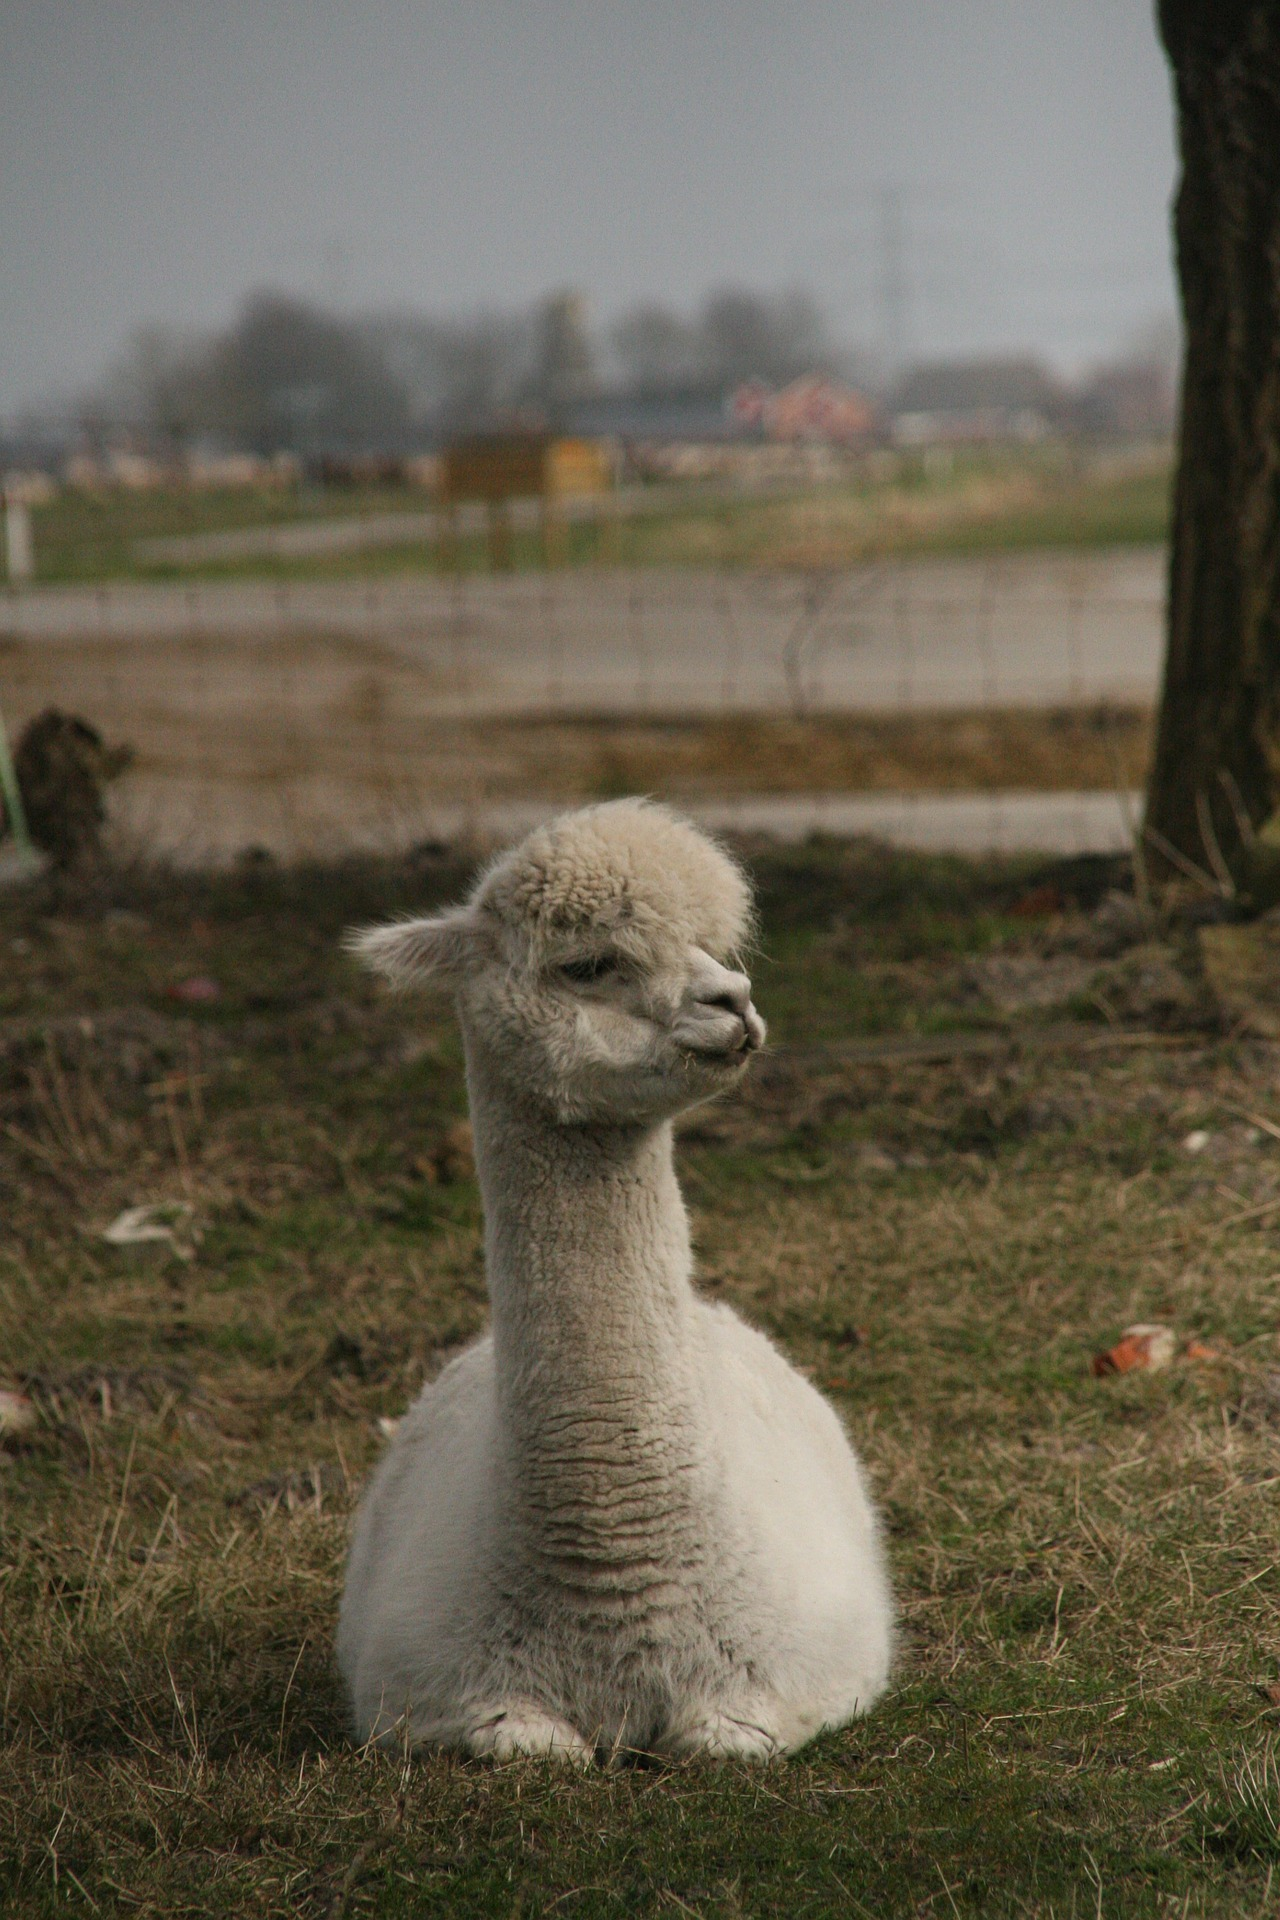
\includegraphics[width=0.3\textwidth]{Figures/placeholder.jpg}
  \caption{Placeholder.} 
  \label{fig:placeholder}
\end{figure}
\cite{jones2001taxonomy} shows an example for a citation in the next, or it can be done like this when it is not included in a sentence \citep{jones2001taxonomy}.


\bibliographystyle{apacite}
\bibliography{literature}

\end{document}
